\chapter{Vulnerability, Attack, Intrusion}
\section{Vulnerability}
A \textbf{vulnerability} is a defect in a person, a component or a set of rules which enables a threat agent to execute an \textbf{attack}:
action that grants access rights that violate the security policy.

In short,
\begin{center}
    \textit{\ul{A \textbf{vulnerability} is a bug that enables an \textbf{attack}}}
\end{center}

\note{\textit{Every} vulnerability is a bug, but \textit{not} every bug is a vulnerability}

\section{Attack}
An \textbf{attack} is an action and/or the execution of some code that may grant to the person or the module that executes it some illegal access rights, and it is related to a vulnerability that enables it.\\
The output of an attack is \textbf{stochastic}, it may fail according to a probability distribution.


\section{Threat Agent}
A \textbf{threat agent} is a source of \textbf{attacks},
it may be \textit{natural} (floodings, earthquakes...) or \textit{man-made }(adversary with a goal).
\textit{Man-made} may be malicious or random (employee which clicks on something dangerous accidentally).

\begin{center}
    It is possible to \textbf{assess risk} only if assets, vulnerabilities and threat agents are known for a given system. 
\end{center}

\section{Intrusion}
An \textbf{intrusion} is a sequence of \textit{actions} and \textit{attacks} of a threat agent to reach its goal,
which initially owns its legal access rights and aims to gain illegal ones,
hoping to control {---} a subset of {---} an ICT/OT system.
Some actions may be actuals attacks, while others may collect information to discover possible attacks.
Such actions (and attacks) can be implemented by a program called \textit{exploit}.

Once a threat agent gained control over an ICT/OT system:
\begin{itemize}
    \item Collect and exfiltrate infomration from the system
    \item Update any information in the system
    \item Prevent access to any resource/information in the system
\end{itemize}
\begin{center}
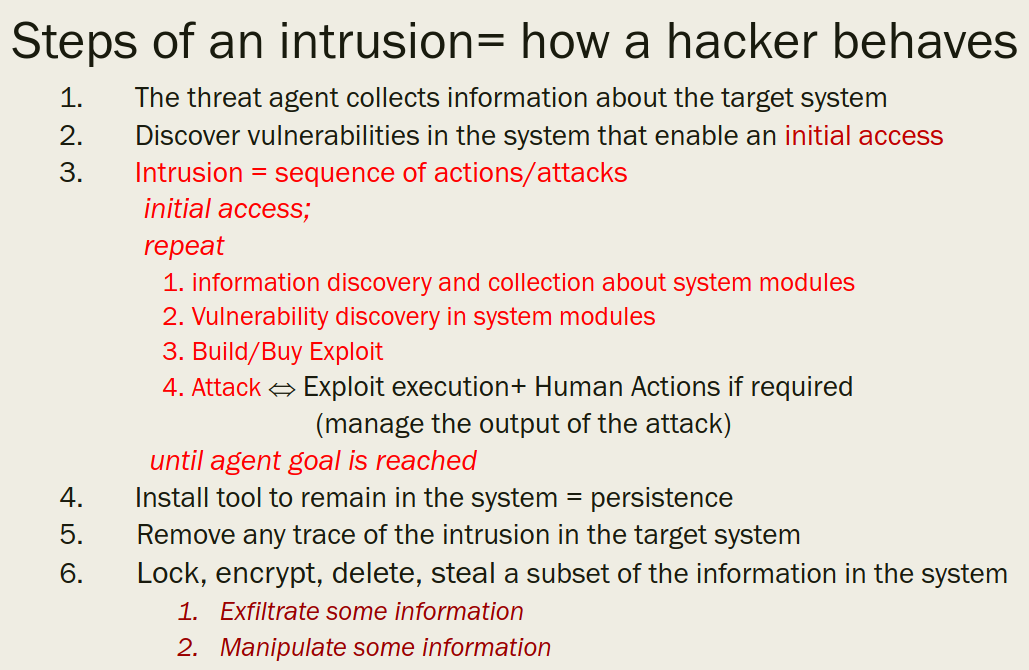
\includegraphics[width=0.7\textwidth]{images/intrusion_steps.png}
\end{center}
The steps of an intrusion include a recursive phase highlighted in \text{\color{red}red} in the picture;
it appears clear that an attacker \textbf{cannot} plan an entire intrusion in advance before starting it,
since an attack reveals information and (possibly) vulenon the system which the next attack will be based on.

\section{Initial Access}
A set of techniques that adversaries may use in an intrusion as entry vectors to gain an initial foothold within an ICT/OT environment.

Informations gathered through initial access are sold on the deep web to hackers team who aim to penetrate a system.\\
Initial Access is a critical step in intrusions.

\section{Countermeasure}
The \textbf{attack chain} is the sequence of \textit{useful} attacks in an intrusion.
A defendant wants to increase the number of \textit{useless} attacks to slow down an intrusion.
Besides, it is not mandatory to remove \textit{all} vulnerabilities to prevent an in intrusion,
but even only one may be sufficient to interrupt te \textit{attack chain}, 
thus preventing the attacker from collecting information that would lead to further attacks.\nl

There are two main approaches when considering security:
\begin{itemize}
    \item \textbf{Unconditional security}: Assume that any vulnerability will be exploited regardless of costs and complexity
    \item \textbf{Conditional security}: Consider who is interested in attacking the system and which vulnerabilities their intrusion can exploit. 
\end{itemize}

\section{Risk assessment}
To wrap up, let's define what \textbf{Risk assessment and management} involves,
keeping in mind that \textit{cyber risk} resembles the average loss for instrusions.
\begin{enumerate}
    \item Asset analysis
    \item Threat agent analysis
    \item Vulnerability analysis
    \item Adversary emulation
    \item Impact analysis
    \item Risk evaluation and management: \textit{compute and minimize loss}
    \begin{itemize}
        \item Compute the risk
        \item Accept some risk
        \item Reduce some risk (countermeasures + scheduling)
        \item Transfer residual risk (insurance)
    \end{itemize}
\end{enumerate}